\newpage
\section{Ergebnisse}
\subsection{100 Würfel Animation}
Für die beiden folgenden Tabellen gilt, dass ein höheres Ergebnis eine bessere Leistung darstellt.
\begin{figure}[H]
    \centering
    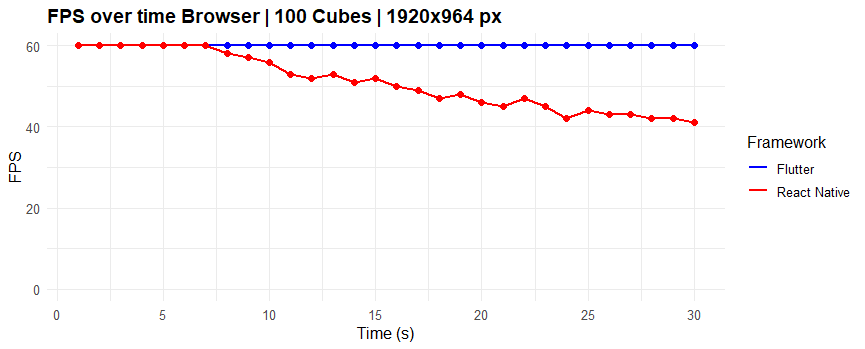
\includegraphics[width=1\linewidth]{images/web/100Cubes.png}
    \caption{FPS über Dauer Web}
\end{figure}

\begin{figure}[H]
    \centering
   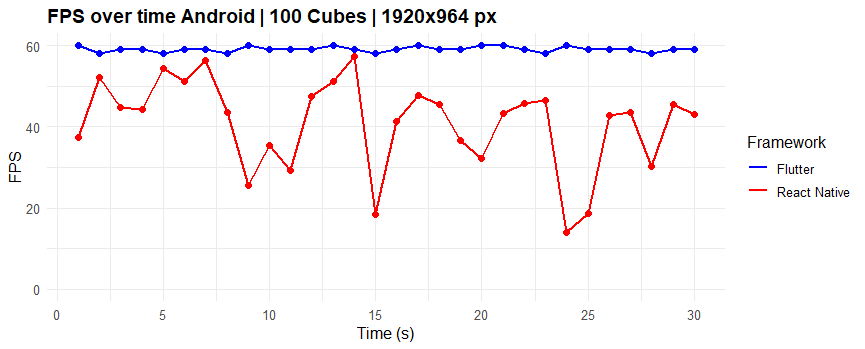
\includegraphics[width=1\linewidth]{images/android/100Cubes.png}
    \caption{FPS über Dauer Android}
\end{figure}

\begin{table}[h!]
    \centering
    \begin{tabular}{llll}
    \toprule
    \textbf{Framework} & \textbf{Plattform} & \textbf{Mittelwert in FPS} & \textbf{Median in FPS} \\
    \midrule
        Flutter & Web & 60 & 60 \\
        Flutter & Android & 59.03 & 59 \\
        React Native & Web & 50.87 & 50.5 \\
        React Native & Android & 40.87 & 43.55 \\
    \bottomrule
    \end{tabular}
\end{table}

Die durchgeführten Tests haben ergeben, dass Flutter in der Lage ist, die Framerate von 60 Bildern pro Sekunde über einen konstanten Zeitraum aufrechtzuerhalten. React Native hingegen hält die 60 FPS bis zur siebten Sekunde stabil, bevor ein langsamer Abfall einsetzt. Auf dem Android-Gerät zeigt Flutter insgesamt eine durchgehend stabile Leistung. Bei der Darstellung von 100 animierten Elementen sind jedoch starke Schwankungen festzustellen, die durch React Native verursacht werden.

Flutter profitiert von seiner plattformunabhängigen Rendering-Engine Skia, die eine direkte und effiziente Darstellung von Animationen ermöglicht. React Native hingegen verwendet den virtuellen DOM und ist von dessen Performance abhängig, wodurch die FPS mit zunehmender Dauer sinken können. Diese Beobachtungen zeigen, dass Flutter in diesem Test performanter ist.

Auf dem Android-Gerät nutzt Flutter ebenfalls seine eigene Rendering-Engine, was zu ähnlichen Ergebnissen wie im Browser führt. React Native muss den JavaScript-Code in die native Sprache übersetzen, was bei vielen Anfragen zu Verzögerungen führt. Allerdings zeigt auch Flutter bei der Darstellung von 100 Würfeln geringfügige Leistungseinbußen.

\newpage
\subsection{1000 Würfel Animation}

\begin{figure}[H]
    \centering
    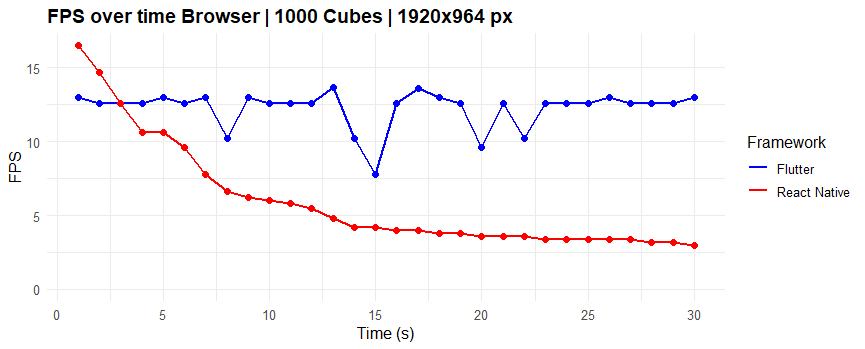
\includegraphics[width=1\linewidth]{images/web/1000Cubes.png}
    \caption{FPS über Dauer Web}
\end{figure}

\begin{figure}[H]
    \centering
    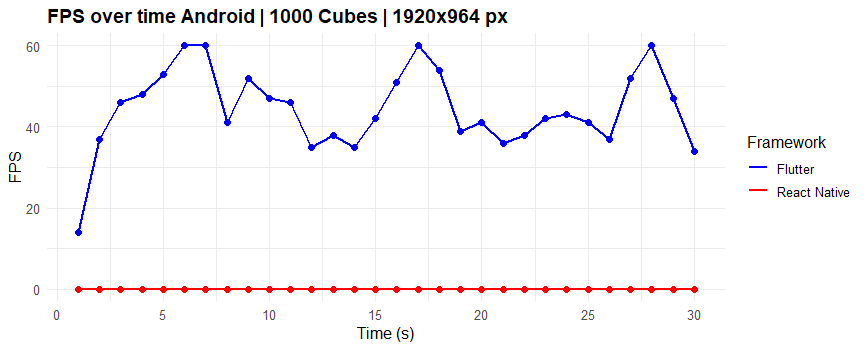
\includegraphics[width=1\linewidth]{images/android/1000Cubes.png}
    \caption{FPS über Dauer Android}
\end{figure}

\begin{table}[h!]
    \centering
    \begin{tabular}{llll}
    \toprule
    \textbf{Framework} & \textbf{Plattform} & \textbf{Mittelwert in FPS} & \textbf{Median in FPS} \\
    \midrule
        Flutter & Web & 12.26 & 12.6 \\
        Flutter & Android & 44.29 & 42.5 \\
        React Native & Web & 5.95 & 4.1 \\
        React Native & Android & 0 & 0 \\
    \bottomrule
    \end{tabular}
\end{table}

Bei 1.000 animierten Würfeln im Browser zeigt Flutter leichte Schwankungen und erzielt FPS im unteren Bereich. React Native erreicht zu Beginn höhere FPS als Flutter, jedoch flacht die Kurve im weiteren Verlauf deutlich ab. Als Android-App zeigt Flutter im Vergleich zur Leistung im Browser eine deutlich bessere Performance. React Native hingegen schafft es bei dieser Anzahl an Elementen nicht, mehr als 0 Bilder pro Sekunde darzustellen.

Mit einer erhöhten Anzahl animierter Elemente erleiden beide Frameworks Leistungseinbußen. Im Browser ist ein geringfügiger Unterschied zu erkennen: Nach einer gewissen Zeit sinkt die Anzahl der Bilder pro Sekunde bei React Native drastisch. Dies ist auf eine Art Stau bei der Manipulation des DOM zurückzuführen.

\newpage
\subsection{Sieb des Erasthenes}
Für diese und folgende Ergebnisse gilt, dass ein niedrigeres Ergebnis eine bessere Leistung darstellt.
\begin{figure}[H]
    \centering
    \includegraphics[width=1\linewidth]{images/web/prime.png}
    \caption{Dauer des Benchmarks im Browser}
\end{figure}

\begin{figure}[H]
    \centering
    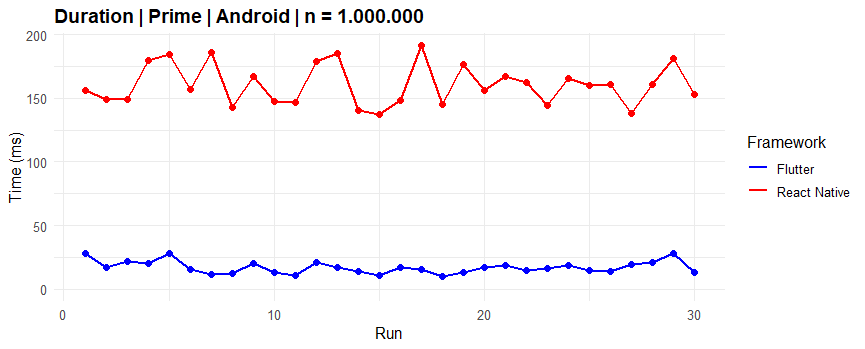
\includegraphics[width=1\linewidth]{images/android/Prime.png}
    \caption{Dauer des Benchmarks im Browser}
\end{figure}

\begin{table}[h!]
    \centering
    \begin{tabular}{llll}
    \toprule
    \textbf{Framework} & \textbf{Plattform} & \textbf{Mittelwert in ms} & \textbf{Median in ms} \\
    \midrule
        Flutter & Web & 4.74 & 4.57 \\
        Flutter & Android & 17.14 & 16.66 \\
        React Native & Web & 7.02 & 6.83 \\
        React Native & Web & 160.72 & 158.61 \\
    \bottomrule
    \end{tabular}
\end{table}

Die in den Abbildungen dargestellten Graphen verdeutlichen, dass auf beiden Plattformen für die Berechnung mit React Native ein höherer Zeitaufwand erforderlich ist. Im Browser zeigen beide Frameworks eine ähnliche Kurve, die einen relativ konstanten Verlauf aufweist.

React Native nutzt für die Berechnung die JavaScript-Engine des Browsers, in diesem Fall V8, während Flutter in der eigenen Dart-VM ausgeführt wird. Der Dart-Code wird mittels AOT-Kompilierung (Ahead-of-Time) direkt auf der Hardware ausgeführt. React Native hingegen führt die Berechnung in der JavaScript-Engine durch, die kontinuierlich einen Interpreter und die JIT-Kompilierung (Just-in-Time) verwendet. Beide Frameworks nutzen JavaScript zur Berechnung der Zahlen, da bei Flutter nur das CanvasKit, welches zur Darstellung von Elementen dient, WebAssembly nutzt.
Die Garbage Collection von Flutter ist speziell auf Dart-Code ausgelegt, was eine inkrementelle und effiziente Speicherverwaltung ermöglicht.

Insgesamt lässt sich feststellen, dass React Native durch verschiedene Eigenschaften wie die dynamische Typisierung, die flexible Array-Verwaltung und die JavaScript-Bridge an Leistung einbüßt.

\newpage
\subsection{State Management}
\begin{figure}[H]
    \centering
    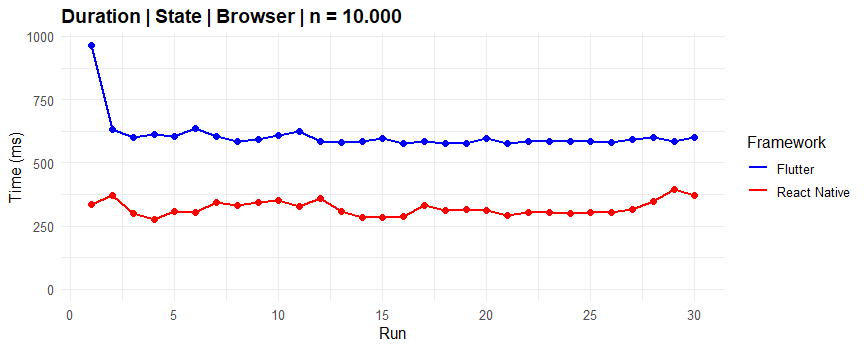
\includegraphics[width=1\linewidth]{images/web/State.png}
    \caption{Dauer des Benchmarks im Browser}
\end{figure}

\begin{figure}[H]
    \centering
    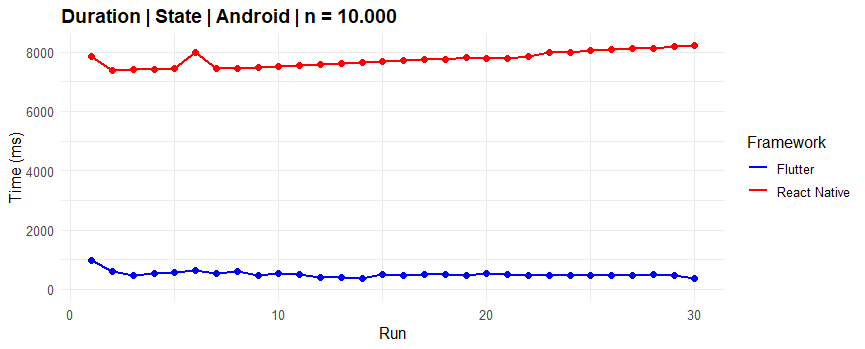
\includegraphics[width=1\linewidth]{images/android/State.png}
    \caption{Dauer des Benchmarks im Browser}
\end{figure}

\begin{table}[h!]
    \centering
    \begin{tabular}{llll}
    \toprule
    \textbf{Framework} & \textbf{Plattform} & \textbf{Mittelwert in ms} & \textbf{Median in ms} \\
    \midrule
        Flutter & Web & 606.13 & 598.67 \\
        Flutter & Android & 506 & 482.16 \\
        React Native & Web & 320.69 & 313 \\
        React Native & Android & 7756.89 & 7762 \\
    \bottomrule
    \end{tabular}
\end{table}

Die Ausführung des Benchmarks erfolgt bei React Native im Browser mit höherer Geschwindigkeit. Beide Graphen zeigen eine konstante Entwicklung, wobei Flutter zu Beginn einen hohen Wert erzielt, der im folgenden Durchlauf deutlich sinkt und danach nahezu konstant bleibt. Als mobile Android-App bleiben die Graphen weiterhin konstant, jedoch erzielt React Native deutlich schlechtere Werte, während Flutter die Messergebnisse verbessert.

Die Geschwindigkeit, mit der Daten in einen State gepackt und wieder daraus gelöscht werden, hängt von der Rendering-Strategie der Frameworks ab. In Flutter Web werden Zustände effizient verarbeitet, jedoch kann der CanvasKit-Renderer bei komplexen Zustandsänderungen zusätzlichen Overhead verursachen, insbesondere bei häufigem UI-Rendering. React Native Web verwendet die JavaScript-Engine des Browsers und aktualisiert das virtuelle DOM, was bei häufigen oder großen Zustandsänderungen zu einer höheren CPU-Belastung führen kann, da das UI bei jeder Änderung neu gerendert wird. Insgesamt kann Flutter bei komplexeren UI-Komponenten langsamer sein, während React Native Web bei häufigen, kleinen Zustandsänderungen aufgrund der virtuellen DOM-Strategie etwas langsamer sein kann.

Auf dem Android-Gerät funktioniert die Kommunikation bei React Native anders: Sämtliche Updates müssen über die Bridge kommuniziert werden. Die Darstellung der Items, die Manipulation der Daten und das Rendern als native Elemente führen zu einer geringeren Leistung. Flutter hingegen ist für mobile Anwendungen optimiert und verwendet Techniken wie AOT-Kompilierung und Widget-Verwaltung, um die Leistung aufrechtzuerhalten.

\newpage
\subsection{Speicher}
\begin{figure}[H]
    \centering
    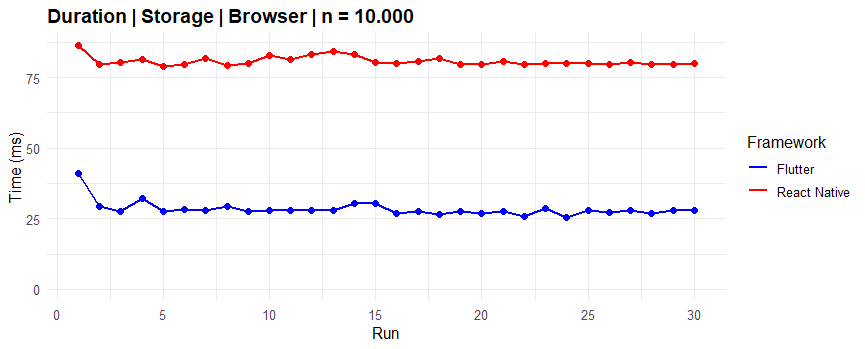
\includegraphics[width=1\linewidth]{images/web/Storage.png}
    \caption{Dauer des Benchmarks im Browser}
\end{figure}

\begin{figure}[H]
    \centering
    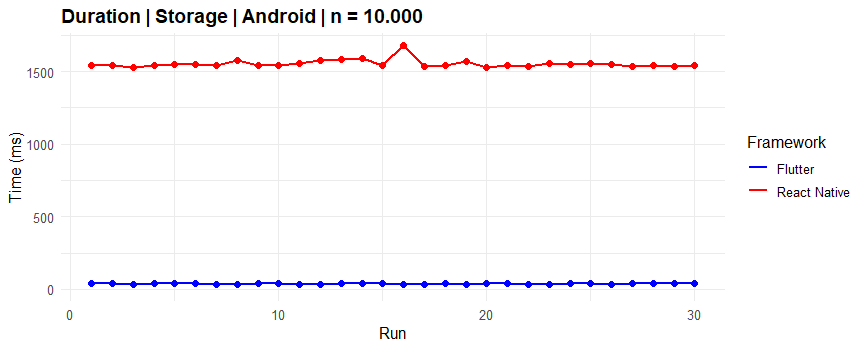
\includegraphics[width=1\linewidth]{images/android/Storage.png}
    \caption{Dauer des Benchmarks im Browser}
\end{figure}

\begin{table}[h!]
    \centering
    \begin{tabular}{llll}
    \toprule
    \textbf{Framework} & \textbf{Plattform} & \textbf{Mittelwert in ms} & \textbf{Median in ms} \\
    \midrule
        Flutter & Web & 28.44 & 28 \\
        Flutter & Android & 37.61 & 37.5 \\
        React Native & Web & 80.82 & 80.09 \\
        React Native & Android & 1553.17 & 1543.83 \\
    \bottomrule
    \end{tabular}
\end{table}


In diesem Test gibt es im Browser bei beiden Frameworks die Gemeinsamkeit, dass sie beide den LocalStorage des Browsers nutzen. React Native Web verwendet ein Polyfill, also eine Bibliothek, die fehlende Funktionen durch alternative Implementierungen bereitstellt, um die Verbindung zum LocalStorage zu ermöglichen. Dies sorgt für Cross-Plattform-Kompatibilität, da derselbe Code sowohl in Web- als auch in nativen Umgebungen funktioniert. Allerdings kann die Verwendung von Polyfills zu Performance-Einbußen führen, da zusätzliche Abstraktionsschichten erforderlich sind, um die Web-API zu emulieren. Flutter Web nutzt ebenfalls JavaScript, um mit Browser-APIs wie LocalStorage zu kommunizieren. Flutter führt den Code nicht direkt auf dem Endgerät aus, sondern transpiliert ihn nach JavaScript, wodurch auch hier keine direkte Kommunikation mit den Web-APIs erfolgt. Daher greifen beide Frameworks auf den LocalStorage zu, allerdings auf unterschiedliche Weise: React Native Web über Polyfills und Flutter Web über JavaScript, ohne Polyfills zu benötigen.

Auf dem Android-Gerät unterscheidet sich die Implementierung der beiden Frameworks. Flutter greift auf die SharedPreferences des Geräts zu, welche für die Speicherung von kleineren Datenmengen optimal sind und zum Großteil synchron sind. React Native nutzt bei der Implementierung eine SQLite-Datenbank, welche die Verwaltung von großen und komplexen Datenmengen verbessert, jedoch für den getesteten Fall einen großen Overhead darstellt. Die Daten werden bei den SharedPreferences als XML-Datei gespeichert, wodurch der Zugriff schnell erfolgt. Bei React Native muss jede Anfrage von Daten über die Datenbank getätigt werden, wodurch es zu Ladezeiten kommt. Das asynchrone Laden von Daten bietet ebenfalls viele Vorteile, hat aber Schwächen bei der Ladezeit.

\newpage

\subsection{Forschungsfragen}
In der Anforderungsanalyse wurde bereits die fundamentale Forschungsfrage mit ihren Unterfragen erwähnt.

\vspace{0.5cm}

\textit{Welche messbaren Unterschiede in der Darstellungsleistung ergeben sich im Vergleich zwischen Flutter und React Native in modernen Cross-Plattform-Anwendungen?}


\begin{enumerate}
    \item Wie unterscheiden sich React Native und Flutter in Render- und Rechenleistung bei typischen Entwicklungsaufgaben?
    \item Gibt es Unterschiede der Leistung auf verschiedenen Endgeräten?
    \item Welches Framework ist für die alltägliche Praxis im Hinblick auf die Leistung attraktiver?
\end{enumerate}


\subsubsection{Beantwortung der Forschungsfrage 1}
Um den quantitativen Unterschied ermitteln zu können, wird die Differenz der Messergebnisse in Abhängigkeit vom Endgerät ermittelt, indem der Mittelwert für den jeweiligen Test von Flutter mit dem Wert von React Native subtrahiert wird.

\begin{table}[h!]
    \centering
    \begin{tabular}{|l|l|p{4cm}|l|}
    \toprule
    \textbf{Benchmark} & \textbf{Platfform} & \textbf{Differenz Flutter React Native}& \textbf{Prozentuale Differenz} \\
    \midrule
    Cube 100   & Web   & 9.13 fps & 17.95 \%       \\
    Cube 100   & Android   & 18.16 fps & 44.43 \%      \\
    Cube 1000  & Web & 6.31 fps & 106.05 \%    \\
    Cube 1000  & Android & 44.29 fps & unendlich \%     \\
    Prime      & Web   & 2.28 ms & 48.12  \%   \\
    Prime      & Android   & 143.58 ms & 838 \%    \\
    State      & Web   & 52.38 ms & 184.05 \%  \\
    State      & Android   & 1515.56 ms & 4033.26 \%   \\
    Storage    & Web   & - 285.44 ms & - 89 \%  \\
    Storage    & Android   & 7250.89 ms & 1434.34 \% \\
    \bottomrule
    \end{tabular}
\end{table}

Die Tabelle zeigt, dass es bei nahezu allen Benchmarks auf allen Endgeräten Leistungsunterschiede gibt, bei denen Flutter die bessere Leistung aufweist. Die einzige Ausnahme ist bei dem Storage Benchmark im Browser, bei dem React Native eine bessere Leistung aufzeigt. Aus diesen Unterschieden lässt sich ableiten, dass Flutter in den getesteten Benchmarks eine bessere Performance im Bereich der Rechen- und Darstellungsleistung aufweist.

\subsubsection{Beantwortung der Forschungsfrage 2}
Die Untersuchung der ersten Forschungsfrage ergab, dass es erhebliche Unterschiede zwischen den einzelnen Frameworks bei der Leistung gibt. Um die Leistungsunterschiede eines Frameworks auf den verschiedenen Geräten zu ermitteln, wird die Differenz der Benchmarks, welche im Browser und auf einem Android-Gerät, berechnet und analysiert. Im Folgenden wird die Differenz der Leistung vom Android-Gerät zum Browser ermittelt und zum Vergleich herangezogen.

\begin{table}[h!]
    \centering
    \begin{tabular}{|l|p{3cm}|p{3cm}|p{3cm}|p{3cm}|}
    \hline
    \textbf{Benchmark} & \textbf{Differenz (Flutter)} & \textbf{Prozentual Flutter} & \textbf{Differenz (React Native)} & \textbf{Prozentual React Native} \\
    \hline
    Cube 100   & 0.97 fps & 1.64 \% & 10 fps & 24.4 \% \\
    Cube 1000  & -32.03 fps & -261.16 \% & 5.95 fps & unendlich \% \\
    Prime      & 12.4 ms & 261.18 \% & 153.7 ms & 2191.56 \% \\
    State      & -100 ms & -19.7 \% & 7436.2 ms & 2320.35 \% \\
    Storage    & 9.71 ms & 32.2 \% & 1472.35 ms & 1822.27 \% \\
    \hline
    \end{tabular}
    \caption{Vergleich der Differenzen und prozentualen Unterschiede zwischen Flutter und React Native Benchmarks}
\end{table}


Anhand der Tabelle lässt sich erkennen, dass es bei React Native in allen Benchmarks zu Ergebnissen kommt, welche belegen, dass die Leistung von React Native auf dem Android-Gerät konstant schlechter ist, als im Browser. Die signifikante Diskrepanz der ermittelten Mittelwerte in Bezug auf React Native lässt die Vermutung zu, dass die Leistung von React Native auf unterschiedlichen Endgeräten erheblich variiert.

Die Auswertungen der Differenzen von Flutter zeigen, dass bei zwei Benchmarks eine bessere Performance auf dem Android-Gerät im Vergleich zum Browser vorliegt. Die sich daraus ergebenden Unterschiede bewegen sich in einem geringen Bereich von maximal 100 Millisekunden bei den Leistungstests. Bei der Darstellung der Würfel gibt es bei einer hohen Anzahl von Würfeln einen Unterschied von bis zu 30 Frames pro Sekunde auf dem Android-Gerät. In der Praxis unter realistischen Bedingungen stellen die Leistungstests keinen merkbaren Unterschied dar. Die Analyse der vorliegenden Daten ergibt, dass die Darstellung und Animation einer hohen Anzahl von Elementen, die 100 nicht überschreitet, keinen signifikanten Unterschied aufweist.

\subsubsection{Beantwortung der Forschungsfrage 3}
Die Benchmarks dieser Arbeit nutzten teilweise für die Praxis unrealistische Bedingungen. Hierzu zählt die große Anzahl an animierten Elementen, sehr häufiges Wechseln des Zustands oder eine Speicherung von unzähligen Daten auf dem Endgerät. Realitätsnähere Werte sorgen für eine geringere Diskrepanz im Vergleich der beiden Frameworks. Dies wurde in einem kleinen Ausschnitt getestet, indem das n der jeweiligen Benchmarks drastisch reduziert und die Ergebnisse in einer Tabelle festgehalten wurden. Es wurden 30 Messungen durchgeführt und die Mittelwerte der Messungen zum Vergleich herangezogen.

\begin{table}[h!]
    \centering
    \begin{tabular}{|l|l|p{3cm}|p{3cm}|p{4cm}|}
    \toprule
    \textbf{Benchmark} & \textbf{Platfform}  & \textbf{Differenz Flutter React Native} & \textbf{Prozentuale Differenz} & \textbf{Mittelwerte Flutter / React Native} \\
    \midrule
    Cube | n = 5   & Web   & 0 fps & 0 \%  & 60 / 60 fps     \\
    Cube | n = 5   & Android   & 0 fps & 0 \% & 60 / 60 fps    \\
    Prime | n = 100      & Web   & 1.467 ms & unendlich \% & 0 / 1.467 ms   \\
    Prime | n = 100      & Android   & 13.961 ms & 305,6 \% & 4.567 / 18.528 ms    \\
    State | n = 10      & Web   & 4.003 ms & 7,76 \% & 52 / 56.033 ms  \\
    State | n = 10      & Android   & 24.788 ms & 47,8 \% & 51.867 / 76.655 ms   \\
    Storage | n = 10    & Web   & 0.003 ms & 1,80 \% & 0.167 / 0.170 ms \\
    Storage | n = 10    & Android   & 2.137 ms & 12,99 \% & 15.767 / 17.815 ms \\
    \bottomrule
    \end{tabular}
\end{table}

Die Tabelle zeigt, dass es nur geringfügige Unterschiede bei den Ergebnissen gibt, welche mit einem kleineren n ermittelt wurden. Eine Differenz von wenigen Millisekunden wird in der Praxis keinen Einfluss auf das Nutzererlebnis haben. Eine Empfehlung für die alltägliche Praxis anhand der Messergebnisse lässt sich bedingt aufstellen, jedoch ist Flutter im Bereich der Leistung ein Stück voraus.

\subsubsection{Beantwortung der fundamentalen Forschungsfrage}
Die fundamentale Forschungsfrage untersucht die messbaren Unterschiede in der Darstellungsleistung zwischen Flutter und React Native in modernen Cross-Plattform-Anwendungen. Die Ergebnisse der Teilfragen zeigen, dass Flutter in den meisten getesteten Benchmarks hinsichtlich der Render- und Rechenleistung überlegen ist. In der ersten Teilfrage wurde deutlich, dass Flutter in nahezu allen Kategorien, wie etwa bei der Darstellung von Würfeln und der Berechnung von Primzahlen, eine bessere Performance bietet. Die einzige Ausnahme bildet der Storage-Benchmark im Browser, bei dem React Native besser abschneidet. In der zweiten Teilfrage wurde festgestellt, dass React Native auf verschiedenen Endgeräten, insbesondere auf Android, eine schlechtere Leistung zeigt als im Browser, während die Leistungsunterschiede von Flutter zwischen den Geräten deutlich geringer ausfallen. In der dritten Teilfrage wurde darauf hingewiesen, dass die getesteten Benchmarks unter teilweise unrealistischen Bedingungen durchgeführt wurden. Unter realistischeren Nutzungsszenarien zeigt Flutter jedoch weiterhin eine bessere Performance. Zusammenfassend lässt sich sagen, dass Flutter im Bereich der Darstellungsleistung und Rechenleistung insgesamt die bessere Wahl ist, insbesondere bei anspruchsvolleren Anwendungen, bei denen Leistung eine entscheidende Rolle spielt.